\documentclass[twoside]{book}

% Packages required by doxygen
\usepackage{fixltx2e}
\usepackage{calc}
\usepackage{doxygen}
\usepackage[export]{adjustbox} % also loads graphicx
\usepackage{graphicx}
\usepackage[utf8]{inputenc}
\usepackage{makeidx}
\usepackage{multicol}
\usepackage{multirow}
\PassOptionsToPackage{warn}{textcomp}
\usepackage{textcomp}
\usepackage[nointegrals]{wasysym}
\usepackage[table]{xcolor}

% Font selection
\usepackage[T1]{fontenc}
\usepackage[scaled=.90]{helvet}
\usepackage{courier}
\usepackage{amssymb}
\usepackage{sectsty}
\renewcommand{\familydefault}{\sfdefault}
\allsectionsfont{%
  \fontseries{bc}\selectfont%
  \color{darkgray}%
}
\renewcommand{\DoxyLabelFont}{%
  \fontseries{bc}\selectfont%
  \color{darkgray}%
}
\newcommand{\+}{\discretionary{\mbox{\scriptsize$\hookleftarrow$}}{}{}}

% Page & text layout
\usepackage{geometry}
\geometry{%
  a4paper,%
  top=2.5cm,%
  bottom=2.5cm,%
  left=2.5cm,%
  right=2.5cm%
}
\tolerance=750
\hfuzz=15pt
\hbadness=750
\setlength{\emergencystretch}{15pt}
\setlength{\parindent}{0cm}
\setlength{\parskip}{3ex plus 2ex minus 2ex}
\makeatletter
\renewcommand{\paragraph}{%
  \@startsection{paragraph}{4}{0ex}{-1.0ex}{1.0ex}{%
    \normalfont\normalsize\bfseries\SS@parafont%
  }%
}
\renewcommand{\subparagraph}{%
  \@startsection{subparagraph}{5}{0ex}{-1.0ex}{1.0ex}{%
    \normalfont\normalsize\bfseries\SS@subparafont%
  }%
}
\makeatother

% Headers & footers
\usepackage{fancyhdr}
\pagestyle{fancyplain}
\fancyhead[LE]{\fancyplain{}{\bfseries\thepage}}
\fancyhead[CE]{\fancyplain{}{}}
\fancyhead[RE]{\fancyplain{}{\bfseries\leftmark}}
\fancyhead[LO]{\fancyplain{}{\bfseries\rightmark}}
\fancyhead[CO]{\fancyplain{}{}}
\fancyhead[RO]{\fancyplain{}{\bfseries\thepage}}
\fancyfoot[LE]{\fancyplain{}{}}
\fancyfoot[CE]{\fancyplain{}{}}
\fancyfoot[RE]{\fancyplain{}{\bfseries\scriptsize Generated by Doxygen }}
\fancyfoot[LO]{\fancyplain{}{\bfseries\scriptsize Generated by Doxygen }}
\fancyfoot[CO]{\fancyplain{}{}}
\fancyfoot[RO]{\fancyplain{}{}}
\renewcommand{\footrulewidth}{0.4pt}
\renewcommand{\chaptermark}[1]{%
  \markboth{#1}{}%
}
\renewcommand{\sectionmark}[1]{%
  \markright{\thesection\ #1}%
}

% Indices & bibliography
\usepackage{natbib}
\usepackage[titles]{tocloft}
\setcounter{tocdepth}{3}
\setcounter{secnumdepth}{5}
\makeindex

% Hyperlinks (required, but should be loaded last)
\usepackage{ifpdf}
\ifpdf
  \usepackage[pdftex,pagebackref=true]{hyperref}
\else
  \usepackage[ps2pdf,pagebackref=true]{hyperref}
\fi
\hypersetup{%
  colorlinks=true,%
  linkcolor=blue,%
  citecolor=blue,%
  unicode%
}

% Custom commands
\newcommand{\clearemptydoublepage}{%
  \newpage{\pagestyle{empty}\cleardoublepage}%
}

\usepackage{caption}
\captionsetup{labelsep=space,justification=centering,font={bf},singlelinecheck=off,skip=4pt,position=top}

%===== C O N T E N T S =====

\begin{document}

% Titlepage & ToC
\hypersetup{pageanchor=false,
             bookmarksnumbered=true,
             pdfencoding=unicode
            }
\pagenumbering{alph}
\begin{titlepage}
\vspace*{7cm}
\begin{center}%
{\Large My Project }\\
\vspace*{1cm}
{\large Generated by Doxygen 1.8.12}\\
\end{center}
\end{titlepage}
\clearemptydoublepage
\pagenumbering{roman}
\tableofcontents
\clearemptydoublepage
\pagenumbering{arabic}
\hypersetup{pageanchor=true}

%--- Begin generated contents ---
\chapter{Hierarchical Index}
\section{Class Hierarchy}
This inheritance list is sorted roughly, but not completely, alphabetically\+:\begin{DoxyCompactList}
\item Q\+Main\+Window\begin{DoxyCompactList}
\item \contentsline{section}{Main\+Window}{\pageref{classMainWindow}}{}
\end{DoxyCompactList}
\item \contentsline{section}{Udp\+Server}{\pageref{classUdpServer}}{}
\item \contentsline{section}{Ui\+\_\+\+Main\+Window}{\pageref{classUi__MainWindow}}{}
\begin{DoxyCompactList}
\item \contentsline{section}{Ui\+:\+:Main\+Window}{\pageref{classUi_1_1MainWindow}}{}
\end{DoxyCompactList}
\end{DoxyCompactList}

\chapter{Class Index}
\section{Class List}
Here are the classes, structs, unions and interfaces with brief descriptions\+:\begin{DoxyCompactList}
\item\contentsline{section}{\hyperlink{classMainWindow}{Main\+Window} \\*The main window for the plot window }{\pageref{classMainWindow}}{}
\item\contentsline{section}{\hyperlink{classUi_1_1MainWindow}{Ui\+::\+Main\+Window} }{\pageref{classUi_1_1MainWindow}}{}
\item\contentsline{section}{\hyperlink{classUdpServer}{Udp\+Server} }{\pageref{classUdpServer}}{}
\item\contentsline{section}{\hyperlink{classUi__MainWindow}{Ui\+\_\+\+Main\+Window} }{\pageref{classUi__MainWindow}}{}
\end{DoxyCompactList}

\chapter{Class Documentation}
\hypertarget{classMainWindow}{}\section{Main\+Window Class Reference}
\label{classMainWindow}\index{Main\+Window@{Main\+Window}}


The main window for the plot window.  


Inheritance diagram for Main\+Window\+:\begin{figure}[H]
\begin{center}
\leavevmode
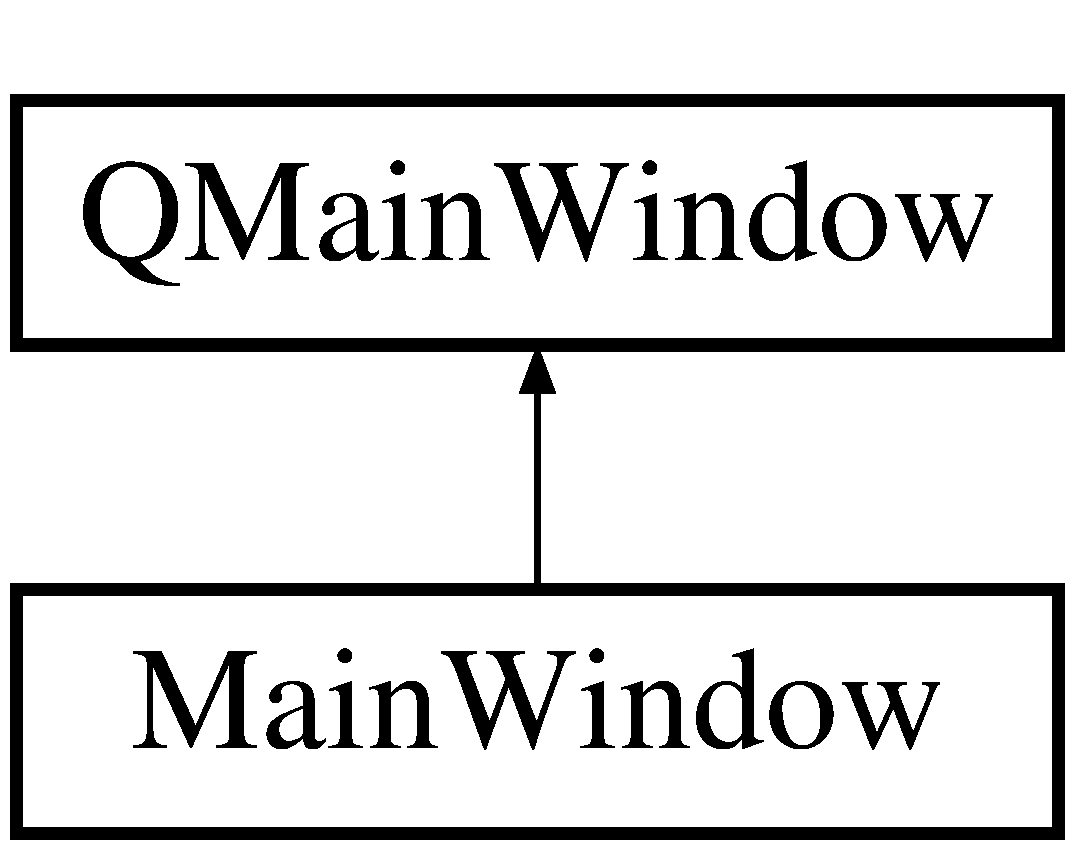
\includegraphics[height=2.000000cm]{classMainWindow}
\end{center}
\end{figure}
\subsection*{Public Member Functions}
\begin{DoxyCompactItemize}
\item 
\hyperlink{classMainWindow_a8b244be8b7b7db1b08de2a2acb9409db}{Main\+Window} (Q\+Widget $\ast$parent=0)
\item 
\hyperlink{classMainWindow_ae98d00a93bc118200eeef9f9bba1dba7}{$\sim$\+Main\+Window} ()
\item 
void {\bfseries start} ()\hypertarget{classMainWindow_a5edcbc314e782645cdf4db101eeb247d}{}\label{classMainWindow_a5edcbc314e782645cdf4db101eeb247d}

\item 
void \hyperlink{classMainWindow_abee37ce669b29d49855fcf5fb76536df}{Run} (Q\+Custom\+Plot $\ast$custom\+Plot, int type)
\end{DoxyCompactItemize}


\subsection{Detailed Description}
The main window for the plot window. 

This \hyperlink{classMainWindow}{Main\+Window} class creates the window that the plot is held in and holds the functions for plotting 

\subsection{Constructor \& Destructor Documentation}
\index{Main\+Window@{Main\+Window}!Main\+Window@{Main\+Window}}
\index{Main\+Window@{Main\+Window}!Main\+Window@{Main\+Window}}
\subsubsection[{\texorpdfstring{Main\+Window(\+Q\+Widget $\ast$parent=0)}{MainWindow(QWidget *parent=0)}}]{\setlength{\rightskip}{0pt plus 5cm}Main\+Window\+::\+Main\+Window (
\begin{DoxyParamCaption}
\item[{Q\+Widget $\ast$}]{parent = {\ttfamily 0}}
\end{DoxyParamCaption}
)\hspace{0.3cm}{\ttfamily [explicit]}}\hypertarget{classMainWindow_a8b244be8b7b7db1b08de2a2acb9409db}{}\label{classMainWindow_a8b244be8b7b7db1b08de2a2acb9409db}
Creates a new \hyperlink{classMainWindow}{Main\+Window} instance, sets up pulseaudio, and begins the plotting \index{Main\+Window@{Main\+Window}!````~Main\+Window@{$\sim$\+Main\+Window}}
\index{````~Main\+Window@{$\sim$\+Main\+Window}!Main\+Window@{Main\+Window}}
\subsubsection[{\texorpdfstring{$\sim$\+Main\+Window()}{~MainWindow()}}]{\setlength{\rightskip}{0pt plus 5cm}Main\+Window\+::$\sim$\+Main\+Window (
\begin{DoxyParamCaption}
{}
\end{DoxyParamCaption}
)}\hypertarget{classMainWindow_ae98d00a93bc118200eeef9f9bba1dba7}{}\label{classMainWindow_ae98d00a93bc118200eeef9f9bba1dba7}
The destructor for \hyperlink{classMainWindow}{Main\+Window} 

\subsection{Member Function Documentation}
\index{Main\+Window@{Main\+Window}!Run@{Run}}
\index{Run@{Run}!Main\+Window@{Main\+Window}}
\subsubsection[{\texorpdfstring{Run(\+Q\+Custom\+Plot $\ast$custom\+Plot, int type)}{Run(QCustomPlot *customPlot, int type)}}]{\setlength{\rightskip}{0pt plus 5cm}void Main\+Window\+::\+Run (
\begin{DoxyParamCaption}
\item[{Q\+Custom\+Plot $\ast$}]{custom\+Plot, }
\item[{int}]{type}
\end{DoxyParamCaption}
)}\hypertarget{classMainWindow_abee37ce669b29d49855fcf5fb76536df}{}\label{classMainWindow_abee37ce669b29d49855fcf5fb76536df}
Runs the plotting of the graph

int type denotes the type of graph that is plotted 

The documentation for this class was generated from the following files\+:\begin{DoxyCompactItemize}
\item 
mainwindow.\+h\item 
mainwindow.\+cpp\end{DoxyCompactItemize}

\hypertarget{classUi_1_1MainWindow}{}\section{Ui\+:\+:Main\+Window Class Reference}
\label{classUi_1_1MainWindow}\index{Ui\+::\+Main\+Window@{Ui\+::\+Main\+Window}}
Inheritance diagram for Ui\+:\+:Main\+Window\+:\begin{figure}[H]
\begin{center}
\leavevmode
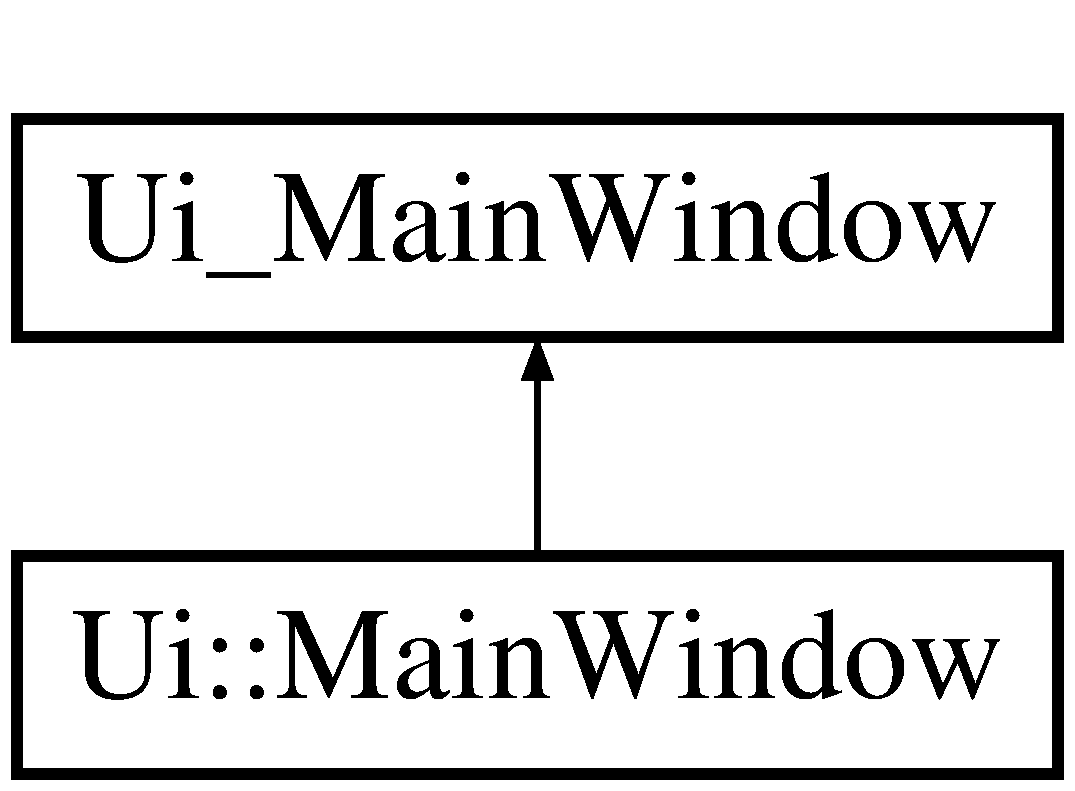
\includegraphics[height=2.000000cm]{classUi_1_1MainWindow}
\end{center}
\end{figure}
\subsection*{Additional Inherited Members}


The documentation for this class was generated from the following file\+:\begin{DoxyCompactItemize}
\item 
ui\+\_\+mainwindow.\+h\end{DoxyCompactItemize}

\hypertarget{classUdpServer}{}\section{Udp\+Server Class Reference}
\label{classUdpServer}\index{Udp\+Server@{Udp\+Server}}
\subsection*{Public Member Functions}
\begin{DoxyCompactItemize}
\item 
{\bfseries Udp\+Server} (char $\ast$to\+Address, int port)\hypertarget{classUdpServer_a85b14ce0beffb7955d7c7ce41a1c92b2}{}\label{classUdpServer_a85b14ce0beffb7955d7c7ce41a1c92b2}

\item 
int {\bfseries set\+Up} ()\hypertarget{classUdpServer_a426f4d98cdb26f8be128a996e8bd55dd}{}\label{classUdpServer_a426f4d98cdb26f8be128a996e8bd55dd}

\item 
void {\bfseries send\+Message} (char message\mbox{[}$\,$\mbox{]})\hypertarget{classUdpServer_a77a3a7cbda482a68b7a63787adc519a7}{}\label{classUdpServer_a77a3a7cbda482a68b7a63787adc519a7}

\item 
void {\bfseries close\+Client} ()\hypertarget{classUdpServer_a7eae90fefc0d563ec814426c0f350201}{}\label{classUdpServer_a7eae90fefc0d563ec814426c0f350201}

\end{DoxyCompactItemize}


The documentation for this class was generated from the following files\+:\begin{DoxyCompactItemize}
\item 
Udp\+Server.\+h\item 
Udp\+Server.\+cpp\end{DoxyCompactItemize}

\hypertarget{classUi__MainWindow}{}\section{Ui\+\_\+\+Main\+Window Class Reference}
\label{classUi__MainWindow}\index{Ui\+\_\+\+Main\+Window@{Ui\+\_\+\+Main\+Window}}
Inheritance diagram for Ui\+\_\+\+Main\+Window\+:\begin{figure}[H]
\begin{center}
\leavevmode
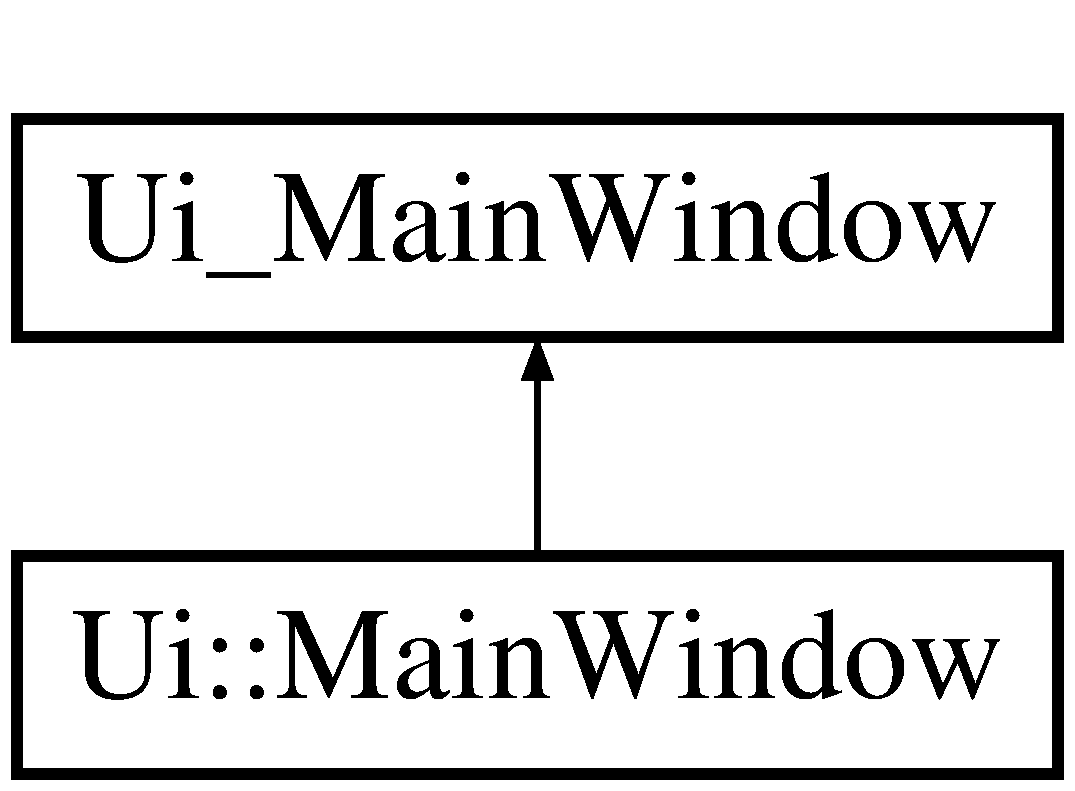
\includegraphics[height=2.000000cm]{classUi__MainWindow}
\end{center}
\end{figure}
\subsection*{Public Member Functions}
\begin{DoxyCompactItemize}
\item 
void {\bfseries setup\+Ui} (Q\+Main\+Window $\ast$\hyperlink{classMainWindow}{Main\+Window})\hypertarget{classUi__MainWindow_acf4a0872c4c77d8f43a2ec66ed849b58}{}\label{classUi__MainWindow_acf4a0872c4c77d8f43a2ec66ed849b58}

\item 
void {\bfseries retranslate\+Ui} (Q\+Main\+Window $\ast$\hyperlink{classMainWindow}{Main\+Window})\hypertarget{classUi__MainWindow_a097dd160c3534a204904cb374412c618}{}\label{classUi__MainWindow_a097dd160c3534a204904cb374412c618}

\end{DoxyCompactItemize}
\subsection*{Public Attributes}
\begin{DoxyCompactItemize}
\item 
Q\+Widget $\ast$ {\bfseries central\+Widget}\hypertarget{classUi__MainWindow_a30075506c2116c3ed4ff25e07ae75f81}{}\label{classUi__MainWindow_a30075506c2116c3ed4ff25e07ae75f81}

\item 
Q\+V\+Box\+Layout $\ast$ {\bfseries vertical\+Layout}\hypertarget{classUi__MainWindow_aecd96a04789fcfec3f98d80390ad8184}{}\label{classUi__MainWindow_aecd96a04789fcfec3f98d80390ad8184}

\item 
Q\+Custom\+Plot $\ast$ {\bfseries custom\+Plot}\hypertarget{classUi__MainWindow_a1e91de1cfe5e44c392cc587158177e7b}{}\label{classUi__MainWindow_a1e91de1cfe5e44c392cc587158177e7b}

\item 
Q\+Status\+Bar $\ast$ {\bfseries status\+Bar}\hypertarget{classUi__MainWindow_a50fa481337604bcc8bf68de18ab16ecd}{}\label{classUi__MainWindow_a50fa481337604bcc8bf68de18ab16ecd}

\end{DoxyCompactItemize}


The documentation for this class was generated from the following file\+:\begin{DoxyCompactItemize}
\item 
ui\+\_\+mainwindow.\+h\end{DoxyCompactItemize}

%--- End generated contents ---

% Index
\backmatter
\newpage
\phantomsection
\clearemptydoublepage
\addcontentsline{toc}{chapter}{Index}
\printindex

\end{document}
